\documentclass[a4paper]{article}
\usepackage{graphicx}
\usepackage[utf8]{inputenc}
\usepackage[english, serbian]{babel}

\title{UseCase: Odabir prihvaćenih radova za tekuće izdanje časopisa}
\date{10.11.2018.}
\author{Dimitrije}

\begin{document}

\maketitle

\begin{itemize}
    \item Akter: Glavni urednik časopisa
    \item Kratak opis: Glavni urednik časopisa razmatra sve radove koji su prihvaćeni i vrši odabir radova koji će ući u tekuće izdanje časopisa.
    \item Osnovni tok događaja:(Ponavljati korake 3, 4, 5. i 6. dok se postigne traženi broj radova ili traženi broj stranica za tekuće izdanje)
        \begin{enumerate}
            \item Glavni urednik upućuje upit sistemu za sve prihvaćene radove koji nisu objavljeni ni u jednom dosadašnjem izdanju časopisa.
            \item Sistem vraća spisak svih takvih radova.
            \item Glavni urednik pregleda sledeći rad.
            \item Glavni urednik donosi odluku da li će rad ući u tekuće izdanje časopisa.
            \item Ukoliko će rad ući u tekuće izdanje: Glavni urednik šalje zahtev sistemu da se rad ubaci u radnu verziju tekućeg izdanja časopisa.
            \item Sistem dodaje rad u radnu verziju tekućeg izdanja.
        \end{enumerate}
    \item Alternativni tok događaja:
        \begin{enumerate}
            \item  (2) Sistem ne vraća uspešno spisak prohvaćenih radova. Glavni urednik pokušava ponovo da izvrši korak 1. Ukoliko ne uspe, obraća se administratoru časopisa.
            \item (3) Sistem ne vraća uspešno sledeći rad koji glavni urednik želi da pregleda. Glavni urednik pokušava ponovo da pregleda rad. Ukoliko ne uspe, obraća se administratoru časopisa.
            \item (6) Sistem ne dodaje rad u radnu verziju tekučeg izdanja. Glavni urednik pokušava ponovo. Ukoliko ne uspe, obraća se administratoru časopisa.
        \end{enumerate}
\end{itemize}

\begin{figure}
    \centering
    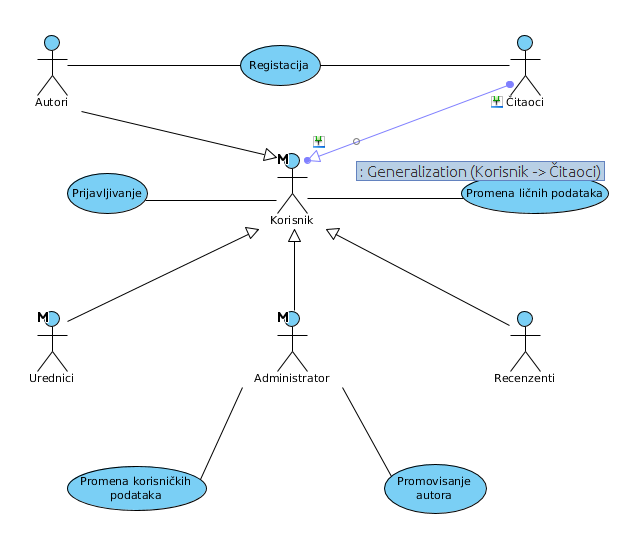
\includegraphics[width=\linewidth]{usecasePrijavljivanje.png}
    \caption{UseCase screenshot}
    \label{fig:my_label}
\end{figure}


\end{document}
